% \documentclass[11pt]{article}
% \usepackage{amsmath}
% \usepackage{graphicx}
% \usepackage[french]{babel}
% \usepackage[utf8]{inputenc}
% \usepackage{fancyhdr}
% \pagestyle{fancy}
%
% \usepackage[left=1.6cm,right=1.6cm,top=2cm,bottom=2cm]{geometry}
%
% \begin{document}
%\fancyhead[L]{Thibaut Heremans - Janvier 2017}
\section{Transformations particulières}
A partir de la différentielle de l'enthalpie  $\mathrm{d}H  = \mathrm{d}U + p \, \mathrm{d}V + V \, \mathrm{d}p$, on peut écrire
$$(C_p - C_v) \mathrm{d}T =  p \, \mathrm{d}V + V \, \mathrm{d}p$$
Avec le premier principe, l'équation des gaz parfaits et la relation de Mayer, on établit :


\begin{table}[!h]
\renewcommand{\arraystretch}{2}
\begin{center}
\begin{tabular}{|r|c|c|c|c|}

  \hline
  & \textbf{Isotherme} & \textbf{Isobare} & \textbf{Isochore} & \textbf{Adiabatique} \\
  \hline
  \hline


  \textbf{Relation}
  & $\mathrm{d}T = 0$
  & $\mathrm{d}p = 0$
  & $\mathrm{d}V = 0$
  & $\displaystyle\frac{p_2}{p_1} = \left( \frac{V_1}{V_2}\right)^\gamma$\\


  & $\displaystyle\frac{\mathrm{d}p}{p} = - \frac{\mathrm{d}V}{V}$
  & $\displaystyle\frac{\mathrm{d}T}{T} = \frac{\mathrm{d}V}{V}$
  & $\displaystyle\frac{\mathrm{d}T}{T} = \frac{\mathrm{d}p}{p}$
  & $\displaystyle\frac{T_2}{T_1} = \left( \frac{V_1}{V_2}\right)^{\gamma-1}$\\


  & $p_1 V_1 = p_2 V_2 $
  & $\displaystyle\frac{T_2}{T_1} = \frac{V_2}{V_1}$
  & $\displaystyle\frac{T_2}{T_1} = \frac{p_2}{p_1}$
  & $\displaystyle\frac{p_2}{p_1} = \left( \frac{T_2}{T_1}\right)^{\frac{\gamma}{\gamma-1}}$\\

\hline

   \textbf{Travail}
   & $W = - \displaystyle \int_{V_1}^{V_2} p  \, \mathrm{d}V $
   & $W = - \displaystyle \int_{V_1}^{V_2} p  \, \mathrm{d}V $
   & $W =0$
   & $W =C_v(T_2-T_1)$ \\

   & $ =- mR^*T \ln \frac{V_2}{V_1} $
   & $ =-p\:(V_2 - V_1)$
   &
   & $ =- \displaystyle\frac{p_1 V_1^\gamma}{1-\gamma}(V_2^{1-\gamma} - V_1^{1-\gamma})$ \\

 \hline

     \textbf{Chaleur}
     & $Q =  -W$
     & $Q = \Delta H = C_p \Delta T$
     & $Q = \Delta U = C_v \Delta T$
     & $Q= 0$\\

  \hline


  &$pV=\textup{cste} $
  &
  &
  &$pV^\gamma=\textup{cste}$
  \\

  \textbf{P,V}
     & 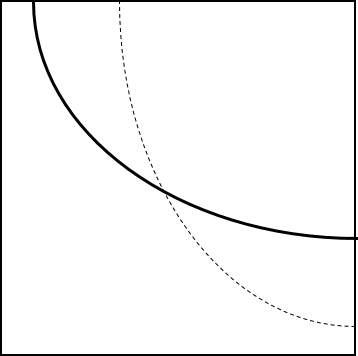
\includegraphics[scale=0.25]{isothermepv.png}
     & 
\includegraphics[scale=0.25]{isobarepv.png}
     & 
\includegraphics[scale=0.25]{isochorepv.png}
     & 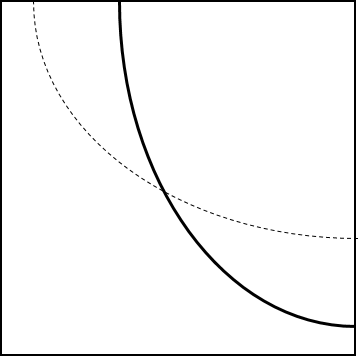
\includegraphics[scale=0.25]{isentropiquepv.png}\\


     \hline

     &
  & $T = T_0 \exp{\frac{S-S_0}{C_p}}$
  & $T = T_0 \exp{\frac{S-S_0}{C_v}}$
  &
  \\

  \textbf{T,S}
     & 
\includegraphics[scale=0.25]{isothermets.png}
     & 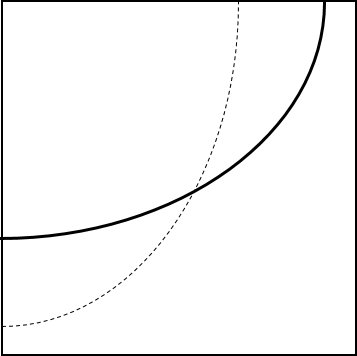
\includegraphics[scale=0.25]{isochorets.png}
     & 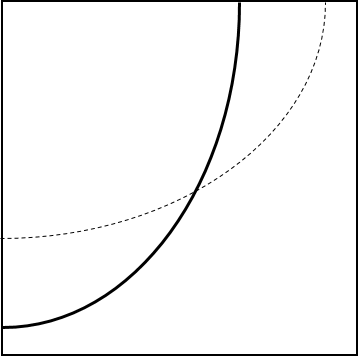
\includegraphics[scale=0.25]{isobarets.png}
     & 
\includegraphics[scale=0.25]{isentropiquets.png}\\



  \hline

\end{tabular}
\end{center}
\end{table}

On remarquera dans les diagrammes (p,V) que l'isotherme est moins raide que l'isentropique (exposant $\gamma$). De manière similaire, l'isochore est plus raide que l'isobare ($C_p > C_V$).
Autres relations utiles dans un cycle :

$$\displaystyle\Delta S = C_v \ln \frac{T_f}{T_i} + m R^* \ln\frac{V_f}{V_i}$$

\[
\left \{
\begin{array}{c @{ = } c}
    C_p - C_v & mR^*=nR \\
    \gamma & \displaystyle\frac{C_p}{C_V} \\
\end{array}
\right.
\]
%\end{document}
